\documentclass[xcolor=table]{beamer}
\usetheme{Madrid}
% \usetheme{Rochester}
% \setbeamertemplate{items}[rectangle]
\usepackage{graphicx} % Required for inserting images
\usepackage{xcolor}
\usepackage{hyperref} %link
\usepackage[normalem]{ulem} % 刪除線email



% --------codeblock-------
\usepackage{listings}
\usepackage{xcolor}

\definecolor{codegreen}{rgb}{0,0.6,0}
\definecolor{codegray}{rgb}{0.5,0.5,0.5}
\definecolor{codepurple}{rgb}{0.58,0,0.82}
\definecolor{backcolour}{rgb}{0.95,0.95,0.92}

\lstdefinestyle{mystyle}{
    backgroundcolor=\color{backcolour},   
    commentstyle=\color{codegreen},
    keywordstyle=\color{blue},
    numberstyle=\tiny\color{codegray},
    stringstyle=\color{codepurple},
    basicstyle=\ttfamily\footnotesize,
    breakatwhitespace=false,         
    breaklines=true,                 
    captionpos=b,                    
    keepspaces=true,                 
    numbers=left,                    
    numbersep=5pt,                  
    showspaces=false,                
    showstringspaces=false,
    showtabs=false,                  
    tabsize=2
}
\lstset{style=mystyle}
% --------中文------------
\usepackage{xeCJK}
%\setmainfont{Times New Roman} %英文字體調整(有時候交中文文件可能有規定對應的英文字體)
\setCJKmainfont{AR PL UKai TW} %中文字體main跟mono都需要哦,最後面的SC是簡體中文,也可以改成TC,不過SC的破字會比較少
\setCJKmonofont{AR PL UKai TW}
\setCJKsansfont{AR PL UKai TW}
\XeTeXlinebreaklocale "zh" %文字間隔
\XeTeXlinebreakskip = 0pt plus 1pt
%-------------------------


\AtBeginSection[]{
  \begin{frame}
    \tableofcontents[currentsection]
  \end{frame}
  \begin{frame}
  \vfill
  \centering
  \begin{beamercolorbox}[sep=6pt,center,shadow=true,rounded=true]{title}
    \usebeamerfont{title}\LARGE\insertsectionhead\par%
  \end{beamercolorbox}
  \vfill
  \end{frame}

}


% 同餘
% 模逆元(模反元素)
% 擴展歐幾里德算法
% 歐拉定理
% 貝祖定理
% 費馬小定理
% 中國餘數定理 (待定) --> 垃圾車
% 質數判斷與篩法
% 調和級數
% sieve of Eratosthenes



\title{競程研討會}
\author{chen910606}
\institute[]{CCUPC} 
\newcommand{\email}{chen910606@gmail.com}
\date{\today}

\begin{document}
\begin{frame}
\titlepage
\end{frame}

\begin{frame}{Outline}
    \tableofcontents 
\end{frame}

\section{出題者的困境}
\begin{frame}{出題者的困境}
    \begin{block}{問題}
         \begin{itemize}
             \item 有 $m$ 題,每題的難度為 $r_i$。
             \item 有 $n$ 個參賽者,每個參賽者的能力值為 $p_i$。
             \item 當參賽者的能力大於等於題目難度時,參賽者會解出那一題題目。
             \item 當比賽滿足對於每個題數,解出恰好該題數的隊伍皆小於等於 $k$ 時代表比賽具有鑑別度。
         \end{itemize}
            試問最少要拿出前幾題才能使比賽具有鑑別度?
    \end{block}
    \vspace{10pt}
    \begin{columns}
        \begin{column}{0.45\textwidth}
            Input\\[1mm]
            4 3 2\\
            400 100 150 200\\
            100 200 300
        \end{column}
        \begin{column}{0.45\textwidth}
            Output\\[1mm]
            3  \vspace{25pt}
        \end{column}
    \end{columns}
\end{frame}

\begin{frame}{出題者的困境-範測解說}
    \begin{columns}
        \begin{column}{0.45\textwidth}
            Input\\[1mm]
            4 3 2\\
            400 100 150 200\\
            100 200 300
        \end{column}
        \begin{column}{0.45\textwidth}
            Output\\[1mm]
            3  \vspace{25pt}
        \end{column}
    \end{columns}
    \vspace{10pt}
    \begin{itemize}
        \item 當 $i = 1$ 時,比賽不具有鑑別度,因為解出 $0$ 題的隊伍有 $3$ 隊。
        \item 當 $i = 2$ 時,比賽不具有鑑別度,因為解出 $1$ 題的隊伍有 $3$ 隊。
        \item 當 $i = 3$ 時,比賽具有鑑別度,因為解出 $0$ 題的隊伍有 $0$ 隊,$1$ 題的有 $1$ 隊,$2$ 題的有 $2$ 隊, $3$ 題的有 $3$ 隊,對於每個題數,其對應的隊伍數皆小於等於 $k$。
    \end{itemize}
\end{frame}

\begin{frame}{出題者的困境 - 觀察}
    \begin{block}{觀察方法}
        \begin{enumerate}
            \item 找出題目不太合理(不符合常理)的地方
            \item 從不合理的點找突破口
        \end{enumerate}
    \end{block}
    \pause
    當參賽者的能力大於等於題目難度時,參賽者會解出那一題題目。\\[3mm]
    
    \pause
    如果把參賽者的能力由小到大排之後,一道題目會把參賽者分成兩部份,左邊為無法答對的組,右邊為可以答對的組。\\[3mm]
    \pause
    兩題不同難度的題目會把參賽者分成三個部份。

\end{frame}

\begin{frame}{出題者的困境 - 觀察}
    
    當一場比賽具有鑑別度時,\\
    再加入一題是否有可能使比賽變成沒有鑑別度?\\[3mm]
    \pause
    % \begin{figure}
    %     \centering
    %     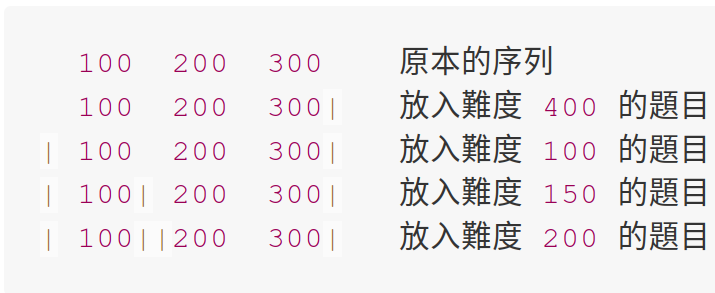
\includegraphics[width=0.5\linewidth]{img/contest_example.png}
        % \caption{}
        % \label{fig:enter-label}
    % \end{figure}
    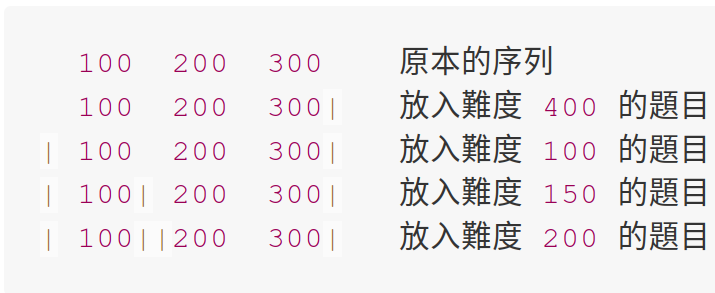
\includegraphics[scale=0.35]{img/contest_example.png}
\end{frame}

\begin{frame}{出題者的困境 - 單調性}
    題數對於鑑別度具有單調性。\\
    可以透過二分搜找答案。\\
    把問題簡化成出前 $x$ 題題目是否有鑑別度。\\[1mm]
    
    \begin{itemize}
        \item 差分
        \item two pointer
    \end{itemize}
\end{frame}

\begin{frame}{出題者的困境 - two pointer}
    
\end{frame}

\end{document}